\documentclass[letterpaper,12pt] {article} 
\usepackage{longtable}
%\usepackage[spanish] {babel} %Paquete para idioma espa�ol
%\usepackage[ansinew] {inputenc}%Gestiona acentos y �
\usepackage{circ}
\usepackage{siunitx}
%\addto\captionsspanish{\renewcommand{\tablename}{Tabla}}					% Cambiar nombre a tablas
%\addto\captionsspanish{\renewcommand{\listtablename}{�ndice de tablas}}		% Cambiar nombre a lista de tablas
\usepackage[T1] {fontenc} 
\usepackage{graphicx} %Paquete para imagenes jpg.
\usepackage {amsmath,amsfonts,amssymb} %Paquete para s�mbolos matem�ticos
\usepackage{float}
\DeclareGraphicsExtensions {.png,.pdf,.jpg}
%\usepackage{circuitikz} %Paquete para dibujar circuitos
\usepackage{tikz}
\usepackage{multirow} %Permite unir varias filas en tablas
\usepackage{multicol} %Permite unir varias columnas en tablas
\usepackage[left=18mm,right=18mm,top=21mm,bottom=21mm] {geometry}
\batchmode
\bibliographystyle{plain} 
\pagestyle{plain} 
\usepackage{pageslts}
\usepackage{lastpage}
\usepackage{fancyhdr}	% Para manejar los encabezados y pies de página
%\renewcommand{\unitvaluesep}{\hspace*{4pt}}	% Redimensionamiento del espacio entre magnitud y unidad
\usepackage[colorlinks=true,urlcolor=blue,linkcolor=black,citecolor=black]{hyperref}     % Para insertar hipervínculos y marcadores
\usepackage{booktabs}	% Para hacer tablas más estilizadas
\usepackage{verbatim}%for commenting blocks 
\usepackage{soul}%for underlining
\usepackage{xcolor}%for changing text color
\usepackage{courier}%for code font
\usepackage{framed}%for boxes

%%%%%%%%%%%%%%%%%%%%
%  for code blocks %
%%%%%%%%%%%%%%%%%%%%
\usepackage[utf8]{inputenc}
\usepackage{listings}
\usepackage{courier}
\definecolor{codegreen}{rgb}{0,0.6,0}
\definecolor{codegray}{rgb}{0.5,0.5,0.5}
\definecolor{codepurple}{rgb}{0.58,0,0.82}
\definecolor{backcolour}{rgb}{0.95,0.95,0.92}

\lstdefinestyle{mystyle}{
	backgroundcolor=\color{backcolour},   
	commentstyle=\color{codegreen},
	keywordstyle=\color{magenta},
	numberstyle=\tiny\color{codegray},
	stringstyle=\color{codepurple},
	basicstyle=\footnotesize\ttfamily,
	breakatwhitespace=false,         
	breaklines=true,                 
	captionpos=b,                    
	keepspaces=true,                 
	numbers=left,                    
	numbersep=5pt,                  
	showspaces=false,                
	showstringspaces=false,
	showtabs=false,                  
	tabsize=2
}

\lstset{style=mystyle}


\author{Jorge Loaiciga, \\{\small Grup}}
\title{{\small  Machine Learning}\\ }
%\date{}  		


\begin{document}
	\pagenumbering{Roman}
	\pagestyle{fancy}		% Contenido de los encabezados y pies de pagina
	\lhead{Embedded Software}
	\chead{}
	\rhead{}
	\lfoot{}
	\cfoot{\thepage}
	\rfoot{}
	
	
%	\pdfbookmark[1]{Portada}{portada} 	% Marcador para el título
	
	\setlength{\unitlength}{1 cm} %Especificar unidad de trabajo
	\thispagestyle{empty}
	\begin{center}
		\textbf{
			{\Huge KAIST}\\[0.5cm]
			%{\LARGE Facultad de Ingeniera }\\[0.5cm]
			{\LARGE Electrical Engineering School}\\[1.75cm]
			{\Large Embedded Software - EE516 }}\\[2.5cm]
			{\LARGE \textbf{Project 5}}\\[2cm]%\\\large{ Control de invernadero.}}
	     	{\LARGE \textbf{"Device Driver for Embedded H/W"}}\\[0.1cm]
	     	{\large Interrupt \& GPIO Control in Beagle Board }\\[2cm]
	     
	     	
	     	{\large Guarav Kalra }\\[0.5cm]
			{\large Mario Loaiciga }\\[0.5cm]
		    {\large Fall Semester - 2016 }\\[1cm] 
		
	\end{center}
	
	\newpage
	
	\pagenumbering{arabic}
	\setcounter{page}{1}
	\pagestyle{fancy}		% Contenido de los encabezados y pies de pagina
	\lhead{Embedded Software - Project 5}
	\chead{}
	\rhead{EE516}
	\lfoot{}\
	
	\cfoot{\thepage}
	\rfoot{}


\section*{Task 1}
\ \ \ \ 
The solution of this first task required of two fundamental structures: \texttt{struct mem\_block}, \texttt{struct linked\_list} (see List. 1). Said structures are combined to allocate memory blocks linked by pointers to other blocks. On module initialization, the function \texttt{dummy\_create()} allocates the required memory for the linked list. For this implementation, we assumed the linked list has a fixed size define as \texttt{LIST\_SIZE} in the \texttt{linked\_list.h} header file. \\


\begin{lstlisting}[firstnumber = 7 ,language=C  ]
typedef struct mem_block
{
	struct mem_block *next;//@ Pointer to next block 
	int value;            //@ Pointer to the value stored in the block

}block;
\end{lstlisting}

\begin{lstlisting}[firstnumber = 14 ,language=C , caption = Linked list structures (included in \texttt{linked\_list.h})  ]
typedef struct linked_list
{
	int cnt;       //@ Number of blocks in the list
	block *head;   //@ Address of first block's structure

}linked_list;
\end{lstlisting}

An extract of the \texttt{dummy\_read()} function is shown in List. 2. This function has the particularity of changing the usage of the argument \texttt{size\_t length}, that is, since the device operates only on fixed size integer values, the read and write functions always return the same amount if bytes. Thus, the  \texttt{size\_t length} argument can now be used by the reader application to communicate to the device driver the value it wants to receive. This behavior can be seen in line 95 of List. 2, where the request is stored in \texttt{rand\_num}. The \texttt{dummy\_read()} function then looks for the request in the list and uses \texttt{copy\_to\_user} to return a value to the user application.\\

The execution of the user space application operating in the linked list memory device is shown in Fig. \ref{task1}. Observe that upon module initialization, the linked list is readied. The application in user space simply obtains the file descriptor of the device \texttt{DUMMY\_DEVICE} and then pass it down to all is threads, which in turn read and write as the semaphores \texttt{sem mutex}, \texttt{sem full} and \texttt{sem empty} allow them to. \\

In the example shown in Fig. \ref{task1}, a total of nine writers start by placing random values the list. Next, three readers request values from the list. The reader with ID 1 requests a value of 1, but since this value was now introduced in the previous write operations, it reads a default value -1. The following two readers obtain their requested values, which were introduced by writer 8 and writer 9. Fig. \ref{task1-r} shows the log of the clean up function which removes the module and also traverses the linked list freeing the allocated memory( \texttt{dummy\_destroy() defined in \texttt{linked\_list.h}}). Notice how in lines 126 and 127 semaphores protect all access to the linked list related structures.  

\newpage
\begin{lstlisting}[firstnumber = 86 ,language=C ]	
ssize_t dummy_read(struct file *file, char *buffer, size_t length, loff_t *offset)
{
\end{lstlisting} 
\begin{lstlisting}[firstnumber = 94 ,language=C , caption = Device read function  ]		
	/*@ Load read value requested from parameter lenght @*/
	rand_num = length;//@ length is now used to request values
	
	down(&full);//@ Sleep if there is zero full blocks
	down(&mutex);//@ Enter criticla region

	/*@ Loop until the hold list has been searched @*/
	while(i < list.cnt){	
		
		if(read_block->value == rand_num){
			
			*dummy_buf = read_block->value;//@ Copy the value to the dummy	
			read_block->value = INIT_VAL;//@ Delete the value from the block
			printk("@ Read HIT\n");
			goto HIT;//@  The value was found, copy to user the value	
		}
		read_block = read_block->next;
		i++;//@ Save the iteartion number
	}
	
	/*@ Else the value was not located, copy -1 to user @*/
	*dummy_buf = INIT_VAL;
	printk(" @ Read MISS\n");
	HIT:		
	if(copy_to_user(buffer, dummy_buf, sizeof(int))){  
		kfree(dummy_buf);
		return -EFAULT;
	}
	
	i = (i>=LIST_SIZE)?-1:i;//@ Block number = -1 if value not found	
	printk("Dummy Driver : Read Call (block: %d, value: %d)\n",i,*dummy_buf);
	
	up(&mutex);//@ Exit critical region
	up(&empty);//@ Signal another block has been emptied
\end{lstlisting}

The operation of the \texttt{dummy\_write()} function has the particularity of using the function \texttt{get\_random\_bytes()} (see List. 3, line 151). This function allows to generate signed random numbers in kernel space. Once the random number is generated, the linked list is traversed again to locate the block to be written. \\ 


\begin{lstlisting}[firstnumber = 136 ,language=C  ]
ssize_t dummy_write(struct file *file,const char *buffer,size_t length,...
{
\end{lstlisting}
\begin{lstlisting}[firstnumber = 142 ,language=C , caption =  Device write function ]	
	block *write_block = list.head;//@ Initialize the block pointer 

	
	if(copy_from_user(dummy_buf, buffer, sizeof(int))){//@ Copy user's data to dummy 
		kfree(dummy_buf);
		return -EFAULT;
	}
	
	/*@ Create random number ( 0 ~ LIST_SIZE-1 )@*/
	get_random_bytes(&rand_num,sizeof(int));
	rand_num = abs(rand_num) % LIST_SIZE;
	
	down(&empty);//@ Sleep if there is zero empty blocks
	down(&mutex);//@ Enter critical region
	
		while( i < rand_num){
			write_block = write_block->next;//@ Trasverse the list until
			i++;                            //@ the random block is pointed at
		}
		
		write_block->value=*dummy_buf;
		
		printk("Dummy Driver : Write Call (block: %d, value: %d)\n",i,*dummy_buf);
		
	up(&mutex);//@ Exit critical region
	up(&full);//@ Signal another block has been filled
\end{lstlisting}








\begin{figure}[H]
	\centering
	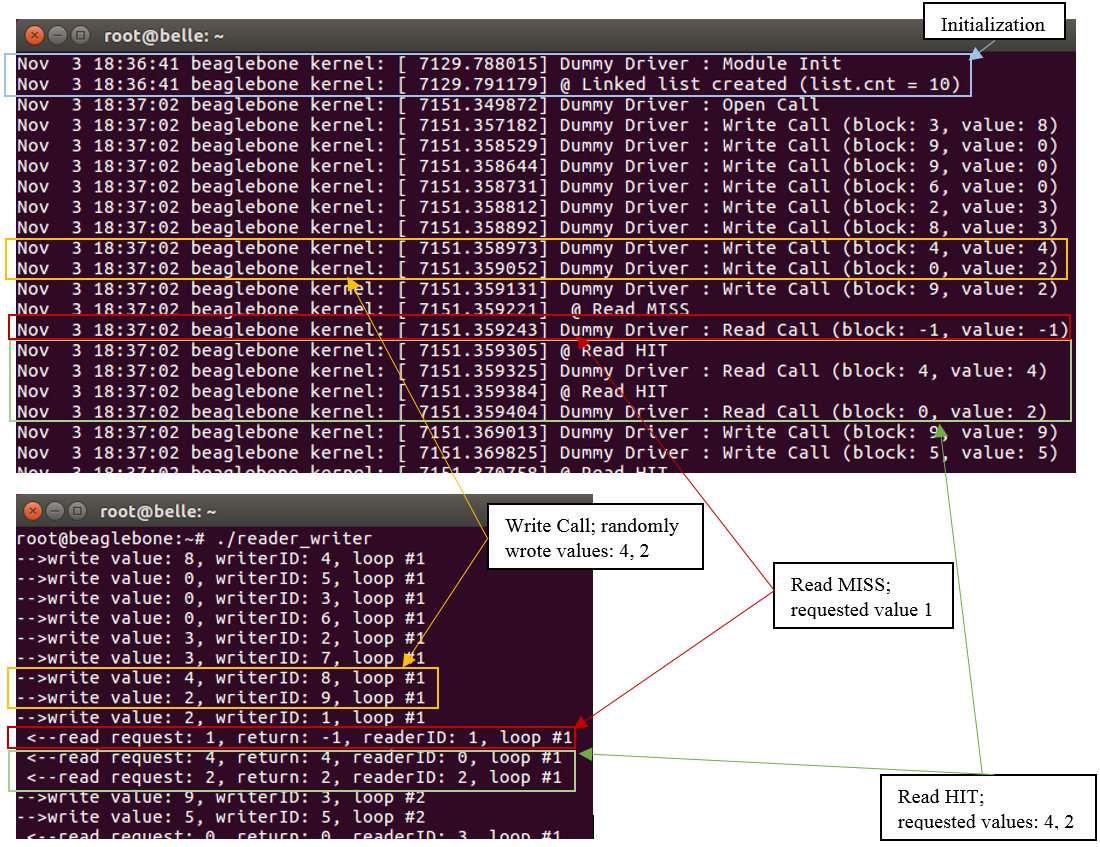
\includegraphics[width=1\textwidth]{task1}\\
	\caption{Linked list module operation}
	\label{task1}
\end{figure}

\begin{figure}[H]
	\centering
	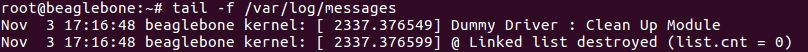
\includegraphics[width=0.9\textwidth]{task1-releas}\\
	\caption{Module unmount and memory clean up}
	\label{task1-r}
\end{figure}



\section*{Task 2}
\ \ \ \
The implementation of this task can be completed progressively building upon the a group of basic functions and structures that allows to handled the  LEDs and create interruptions from both the kernel timers or physical inputs. All the four sub-tasks depend of \texttt{struct gpio\_data}, a structure that holds the reference information of the LEDs (see List. 4). This structured is used to request, by means of a standard procedure, the control over this set of GPIO elements.\\
  
\begin{lstlisting}[firstnumber = 41 ,language=C , caption =  GPIO LED structure for signal mapping  ]
static struct {
		unsigned int gpio; /* GPIO of LED */
		const char *label; /* GPIO label */
		bool valid; /* If TRUE, GPIO is requested & allocated */
	} gpio_data[NUM_LED] = {
			[LED0] = {LED0_GPIO, "LED0_GPIO", FALSE},
			[LED1] = {LED1_GPIO, "LED1_GPIO", FALSE},
			[LED2] = {LED2_GPIO, "LED2_GPIO", FALSE},
			[LED3] = {LED3_GPIO, "LED3_GPIO", FALSE},
};
\end{lstlisting}



\subsection*{Task 2.1} 

The completion of this task depends on the following GPIO functions:

\begin{list}{}{}
	\item \texttt{gpio\_is\_valid()}
	\item \texttt{gpio\_request()}
	\item \texttt{gpio\_direction\_output()}
	\item \texttt{gpio\_set\_value()}
	\item \texttt{gpio\_free()}
\end{list}  

This fairly simple sub-task's operation flow is shown in List. 6. In order to request the GPIO of the LEDs, the costume function  \texttt{\_bb\_module\_startup()} is used. After the LED request is successful, the program turn on the LEDs, one after the other, using the \texttt{gpio\_set\_value()} function which is it at the core of the function \texttt{\_turn\_on\_led()}. This is function is called in each one of the four LEDs.\\

\begin{lstlisting}[firstnumber = 126 ,language=C   ]
static int __init
bb_module_init(void)
{	
	dbg("");
	
	/* startup */
	_bb_module_startup();
	
	/* turn on LED 0 */
	_turn_on_led(LED0_GPIO);
	msleep(1000); //sleep
\end{lstlisting}
\begin{lstlisting}[firstnumber = 146 ,language=C , caption =  Turn on LEDs in sequence  ]	
	/* turn on LED 3 */
	_turn_on_led(LED3_GPIO);
	msleep(1000); //sleep
	
	return 0;
}
\end{lstlisting}


\subsection*{Task 2.2}

The completion of this task depends on the creation of kernel timer interrupts. This is achieved by means of the following functions:

\begin{list}{}{}
	\item \texttt{init\_timer()}
	\item \texttt{add\_timer()}
	\item \texttt{del\_timer()}
	\item \texttt{get\_jiffies\_64()}
\end{list} 

The code is also dependent of the \texttt{struct timer\_list}, defined in \texttt{linux/timer.h}.\\
\begin{lstlisting}[firstnumber = 61 ,language=C    ]
static struct timer_list kern_timer;
\end{lstlisting}

Said structure contains the value \texttt{expires} which is used to save the life time of the timer, as well as a pointer for a function handler that allows us specify an action upon time lapse completion. This structure also contain a value \texttt{data} that can be passed as an argument for later usage. \\

As was the case for the module initialization of the last sub-task, the module first registers GPIO elements and then turns on the LEDs, but now the latter accion is carried out by the \texttt{\_bb\_module\_register\_timer} (see List. 6)\\  

\begin{lstlisting}[firstnumber = 189 ,language=C , caption = Turn LEDs on kernel interrupt   ]
static int __init
bb_module_init(void)
{	
	dbg("");

	/* startup */
	_bb_module_startup();
	
	/* register timer */
	_bb_module_register_timer();
	
	return 0;
}
\end{lstlisting}

List. 7 show the sequence of steps used to register the kernel timer, setting up its expiration time and the eventual callback to the \texttt{kern\_timer\_handler}, a function toggles the state of the LEDs (LED blink).\\

\begin{lstlisting}[firstnumber = 138 ,language=C , caption =  Handling of the timer for kernel interrupts   ]
static void
_bb_module_register_timer(void)
{
	// initialize timer
	init_timer(&kern_timer);
	
	//expire at current + TIME_STEP
	kern_timer.expires = get_jiffies_64() + TIME_STEP;
	
	// handler
	kern_timer.function = kern_timer_handler;
	kern_timer.data = 0;
	
	// add to kernel
	add_timer(&kern_timer);
}
\end{lstlisting}

\subsection*{Task 2.3}
\ \ \ \
The completion of this task depends on the utilization of the following functions interruption request \& handling functions and flags:
\begin{multicols}{2}
		\begin{itemize}
			\item[] \texttt{gpio\_to\_irq()}
			\item[] \texttt{request\_irq()}
			\item[] \texttt{free\_irq()}
			\item[] \texttt{IRQF\_TRIGGER\_RISING}
			\item[] \texttt{IRQF\_TRIGGER\_FALLING}
			\item[] \texttt{IRQF\_TRIGGER\_RISING}
		\end{itemize}
\end{multicols}

In addition, we now introduce the value \texttt{irq\_number} which will serve us to map the GPIO button signal to a IRQ signal in the kernel:\\

\begin{lstlisting}[firstnumber = 63 ,language=C    ]
static unsigned int irq_number;
\end{lstlisting}

Once more, we can see the module initialization (see List. 8) requests the GPIO of the LEDs though \texttt{\_bb\_module\_startup()}. However, now the \texttt{\_bb\_module\_register\_button()} function is introduce to map the GPIO button to a signal interrupt and include an interruption handler that we have called \texttt{button\_irq\_handler()}.\\


\begin{lstlisting}[firstnumber = 300 ,language=C , caption =  Introduction of GPIO interrupt   ]
static int __init
bb_module_init(void)
{
	int ret;
	dbg("");
	
	/* register button */
	ret = _bb_module_register_button();
	if (ret < 0) {
		err("Failed to setup button IRQ");
		return -1;
	}
	
	/* startup */
	_bb_module_startup();
	
	return 0;
}
\end{lstlisting}

In List. 9 we have shown the code of the \texttt{button\_irq\_handler()}. Naturally, this callback function is executed on each rising edge of the GPIO button (\texttt{IRQF\_TRIGGER\_RISING}). The handler carries tow critical tasks: 
\begin{enumerate}
\item Check the current state of the GPIO 
\item Register the kernel timer which will later make the LEDs blink 
\end{enumerate}

\begin{lstlisting}[firstnumber = 193 ,language=C , caption =  GPIO Interruption handling function   ]
static irq_handler_t button_irq_handler
(unsigned int irq, void *dev_id, struct pt_regs *regs)
{
	static bool blinking = FALSE;
	int iter;
	
	// if not blinking, start blinking
	if (blinking == FALSE) {
		/* turn on all LEDs (for quick response) */
		for (iter = LED0; iter < NUM_LED; iter++) {
			// turn on LED
			_turn_on_led(gpio_data[iter].gpio);
		}
		
		/* start pattern */
		_bb_module_register_timer();
		blinking = TRUE;
	}
	// blinking, stop blinking
	else {
		_bb_module_unregister_timer();
		
		/* turn off all LEDs (if still on) */
		for (iter = LED0; iter < NUM_LED; iter++) {
			// if on
			if (!!gpio_get_value(gpio_data[iter].gpio)) {
				// turn off LED
				_turn_off_led(gpio_data[iter].gpio);
			}
		}
		
		blinking = FALSE;
	}
	
	return (irq_handler_t)IRQ_HANDLED;
}
\end{lstlisting}


\subsection*{Task 2.4} 
  
\begin{lstlisting}[firstnumber = 64 ,language=C   ]
static unsigned int counter;

static spinlock_t gpio_press_time_lock;
static ktime_t gpio_press_time;
\end{lstlisting}

\begin{lstlisting}[firstnumber = 291 ,language=C , caption =   GIPO interruption: Detects duration between rising edges  ]
static irq_handler_t button_irq_handler
(unsigned int irq, void *dev_id, struct pt_regs *regs)
{
	uint8_t value;
	unsigned int duration;
	
	spin_lock(&gpio_press_time_lock);
	value = gpio_get_value(BUTTON_GPIO);
	
	if (value == 1) {
		// If no time has elapsed, we probably already cleared on a FALLING
		// interrupt. So finish the handler.
		if (ktime_to_ms(gpio_press_time) == 0) {
			goto finished;
		}
		
		duration = ktime_to_ms(ktime_sub(ktime_get(), gpio_press_time));
		
		if (duration == 0) {
			goto finished;
		}
		
		gpio_press_time = ktime_set(0, 0);
		info("Detected button release, duration of %u", duration);
		
		if (duration >= 1000) { //1sec => reset
			_handle_counter_pattern(TRUE);
		} else {
			_handle_counter_pattern(FALSE);
		}
	} else {
		// If a time is already set, we already received a RISING interrupt.
		// So we can finish the handler.
		if (ktime_to_ms(gpio_press_time) > 0) {
			goto finished;
		}
		
		info("Detected button press");
		gpio_press_time = ktime_get();
	}
	
	finished:
	spin_unlock(&gpio_press_time_lock);
	return (irq_handler_t)IRQ_HANDLED;
}
\end{lstlisting}

\begin{lstlisting}[firstnumber = 263 ,language=C , caption = LED and kernel timer handling    ]
static void
_handle_counter_pattern(bool reset)
{
	unsigned int val;
	static bool timer_registered = FALSE;
	
	val = reset ? _reset_counter_value() : _increment_counter_value();
	
	/* for quick response */
	_turn_on_led_pattern(val);
	
	/* start blinking pattern */
	if (timer_registered == FALSE && val != 0) {
		_bb_module_register_timer();
		timer_registered = TRUE;
	}
	/* value has been reset (remove timer since all LEDs are off anyways) */
	else if (val == 0 && timer_registered == TRUE) {
		_bb_module_unregister_timer();
		timer_registered = FALSE;
	}
	/* renew timer */
	else if (timer_registered == TRUE) {
		_bb_module_unregister_timer();
		_bb_module_register_timer();
	}
}
\end{lstlisting}


\newpage
%
%\begin{thebibliography}{X}
%
%\bibitem{code} . Emin Martinians' Home Page, Red-Black Tree C Code. Signals, Informatino, and Algorithms Group Massachusetts Institute of Technolgy. Available at \href{http://web.mit.edu/~emin/Desktop/ref_to_emin/www.old/source_code/red_black_tree/index.html}{http://web.mit.edu/~emin/Desktop/ref\_to\_emin/www.old/source\_code/red\_black\_tree/index.html}. Consulted on 12/1/16.	
%
% \bibitem{kernel} Love, R. (2005). Linux Kernel Development, 3rd Ed. Indianapolis: Sams Publishing
%
% \bibitem{kernel}Bovet, D. \& Cesati, M. (2000). Understanding the Linux Kernel, 3rd Ed. O'Reilly Media. 

%\begin{thebibliography}{X}
	
%	 \bibitem{chap5} Rusling, D. (1999). The Linux Kernel. Available in \href{http://www.tldp.org/LDP/tlk/ipc/ipc.html}{http://www.tldp.org/LDP/tlk/ipc/ipc.html}. Consulted on 11/07/16.	
%
%	 \bibitem{posix} Salzman, P. (2001). The Linux Kernel Module Programming Guide. Available in \href{https://linux.die.net/lkmpg/}{https://linux.die.net/lkmpg/}. Consulted on 11/06/16.	
%	
%	\bibitem{man} Linux Manual pages (HTML rendereing created by Michael Kerrisk). Available in \href{http://man7.org/linux/man-pages/man7/svipc.7.html}{http://man7.org/linux/man-pages/man7/svipc.7.html}. Consulted on 11/06/16. 
%	
%	\bibitem{unix}Steven, W. et. al.(2003). UNIX Network Programming. Electronic version available in \href{https://scoecomp.files.wordpress.com/2014/02/2003-unix-network-programming-vol-1-3rd-ed.pdf}{https://scoecomp.files.wordpress.com/2014/02/2003-unix-network-programming-vol-1-3rd-ed.pdf}. Consulted on 11/8/16
%
%	\bibitem{really} O'Reilly Linux Documentation Available on\\ \href{http://www.linuxdevcenter.com/pub/a/linux/2007/05/24/semaphores-in-linux.html?page=4}{http://www.linuxdevcenter.com/pub/a/linux/2007/05/24/semaphores-in-linux.html?page=4}.\\Consulted on 11/9/16.
%
%	\bibitem{kernel} Love. R. (2005). Linux Kernel Development. Electronic version available in \href{http://www.makelinux.net/books/lkd2/?u=ch05lev1sec6	}{http://www.makelinux.net/books/lkd2/?u=ch05lev1sec6	}. Consulted on 11/9/16
%\end{thebibliography}
\end{document}
